\documentclass[12pt]{article}

% --- Preamble ---
\usepackage[utf8]{inputenc}
\usepackage[T1]{fontenc}
\usepackage{lmodern}
\usepackage{amsmath, amssymb}
\usepackage{graphicx}
\usepackage{geometry}
\geometry{a4paper, margin=1in}
\usepackage{hyperref} % For clickable links
\usepackage{caption} % For figure and table captions
\usepackage{subcaption} % For subfigures

% --- Document Information ---
\title{Research Report Title}
\author{Your Name(s) \\ Your Affiliation(s) \\ Your Email Address(es)}
\date{\today}

% --- Abstract Environment ---
\usepackage{abstract}
\renewcommand{\abstractname}{Abstract}

% --- Sections and Subsections ---
\setcounter{secnumdepth}{2} % Number up to subsections
\setcounter{tocdepth}{2}    % Include up to subsections in the table of contents

% --- Begin Document ---
\begin{document}

% --- Title Page ---
\maketitle
\begin{abstract}
This section provides a concise summary of your research report. It should briefly outline the problem, the methods used, the key findings, and the main conclusions. Keep it brief and impactful.
\end{abstract}

% --- Table of Contents ---
\tableofcontents
\newpage

% --- Introduction ---
\section{Introduction}
\label{sec:introduction}
This section should introduce the research topic, provide necessary background information, state the problem or research question, and outline the objectives and scope of the report.

% --- Methods ---
\section{Methods}
\label{sec:methods}

\subsection{Participants}
\label{subsec:participants}
This study draws on survey responses from a total of 43 college students, most of whom were enrolled at the University of Florida. While demographic details such as age and gender were not collected, participants were asked to identify their academic major by selecting from one of six broad categories: Engineering, Business, Liberal Arts and Sciences, Health Professions, Law Professions, and Agriculture. These groupings were chosen to represent a wide range of academic disciplines, although a limitation of this approach is that several distinct majors were aggregated into generalized categories. This may obscure more specific differences in AI usage patterns between majors within the same category.

\subsection{Instruments}
\label{subsec:instruments}
To investigate the central research question—how AI usage patterns vary among college students across academic disciplines—we designed a survey aimed at gathering both quantitative and qualitative data. The survey consisted of five questions developed to assess students’ frequency of AI usage, the types of tools they employ, the academic purposes for which they use AI, and their general attitudes and perceptions toward AI in educational contexts.
The first question asked students to indicate their academic discipline by selecting one of the six aforementioned categories. The second question asked students to indicate how often they use AI tools for academic purposes, using a five-point Likert scale that ranged from 'never' to 'nearly every day. The third question allowed students to select from a range of AI tools and services they had used in academic contexts, such as writing assistance, productivity, or study aids. The fourth question asked students to identify the specific academic tasks for which they had used AI, which could include writing assignments, coding, studying for exams, or conducting research. The final question asked students to respond to a series of statements on a five-point Likert scale, where one represented strong disagreement and five represented strong agreement. These statements assessed students’ perceptions of AI’s impact on their learning experience, their access to AI tools, and whether they believe AI is especially useful in their specific field of study.
These questions were selected to help identify trends in AI usage across and within academic fields, reveal which disciplines demonstrate higher engagement with AI tools, and provide insight into how students perceive AI’s usefulness, accessibility, and relevance to their academic work. The survey was intentionally designed to capture both behavior and perception, allowing for a more comprehensive understanding of student interaction with AI in the academic setting. A full copy of the survey instrument is provided in the Appendix.

\subsection{Procedure}
\label{subsec:procedure}
The survey was created using Qualtrics. It was distributed electronically over the course of one week, using university-affiliated group chats and popular social media platforms. The goal was to maximize reach across various academic programs and ensure that students from different disciplines were aware of the study and encouraged to participate.
After an initial round of distribution, it became clear that a large proportion of respondents came from engineering majors. In response to this imbalance, the team made deliberate efforts to reach students in the other disciplines outlined above. Despite these efforts, responses remained heavily skewed, with 46 percent of participants identifying as engineering majors. This overrepresentation presents a limitation in the generalizability of the findings and was taken into account during the analysis.
After the data collection period concluded, the research team performed data cleaning and analysis using both Qualtrics and Python’s Pandas library. These tools allowed for a deeper exploration of the survey responses, enabling the team to identify patterns in AI usage, assess variations in student perceptions across academic disciplines, and draw informed conclusions about how AI tools are being incorporated into students’ academic routines. To facilitate comparisons between disciplines, the data was grouped by major category in Pandas and analyzed to highlight any notable differences in usage patterns and attitudes.

% --- Results ---
\section{Results}
A total of 43 students responded to the survey, though not every participant answered every question. As a result, individual questions received between 37 and 43 responses. Among all respondents, 18 identified as Engineering majors, 11 as Liberal Arts and Sciences majors, 5 as Business majors, and 5 as Health Professions majors. The remaining 4 indicated that none of the listed categories described their major. This distribution is shown in Figure 1. 

\begin{figure}[htbp]
  \centering
  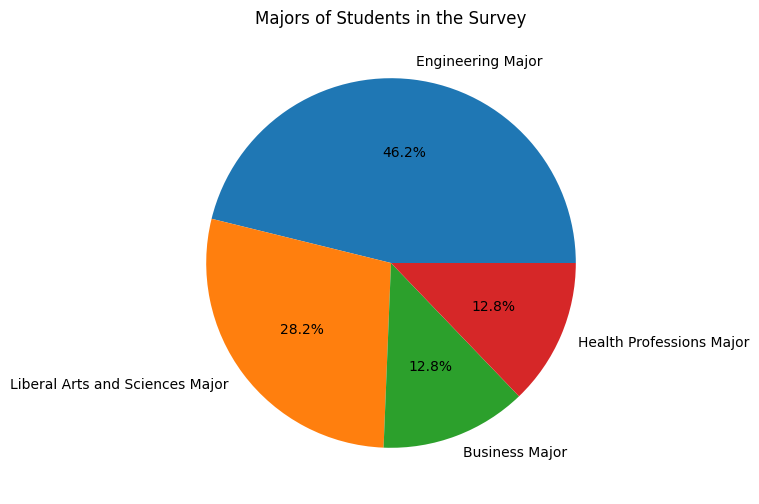
\includegraphics[width=0.5\textwidth]{fig1.png} % Replace with your figure file name
  \caption{A brief description of the figure.}
  \label{fig:example1}
\end{figure}

In response to the question about the frequency of AI tool use for academic purposes, all respondents indicated some level of regular use. The most common response was “a few times per week,” selected by 15 participants. This was followed by “nearly every day” (9 respondents), “daily” (7 respondents), and “at least once a week” (7 respondents). No respondents selected “never” or “a few times a month.” These responses are summarized in Figure 2. 

\begin{figure}[htbp]
  \centering
  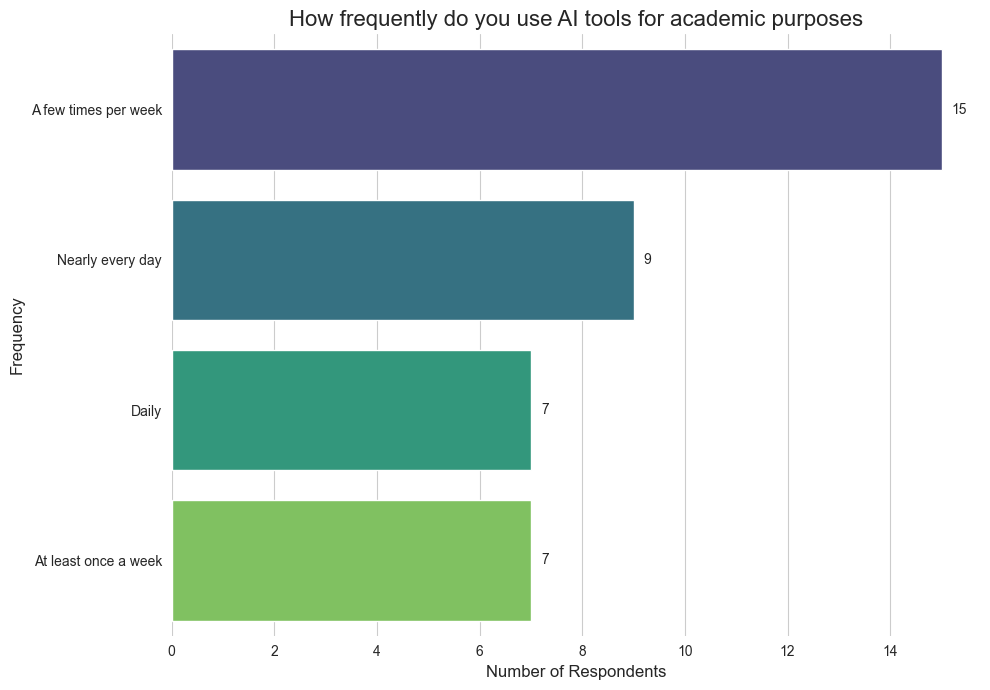
\includegraphics[width=0.6\textwidth]{fig2.png} % Replace with your figure file name
  \caption{A brief description of the figure.}
  \label{fig:example1}
\end{figure}

When asked to select all AI tools and services used for academic purposes, 97\% (38 respondents) reported using ChatGPT, making it the most commonly used tool. Gemini was selected by 46\% (18 respondents), Grammarly AI by 26\% (10 respondents), Claude by 23\% (9 respondents), DALL-E by 15\% (6 respondents), DeepSeek by 13\% (5 respondents), and both Grok and GitHub Copilot by 3\% (1 respondent each). These trends are visualized in Figure 3. 

\begin{figure}[htbp]
  \centering
  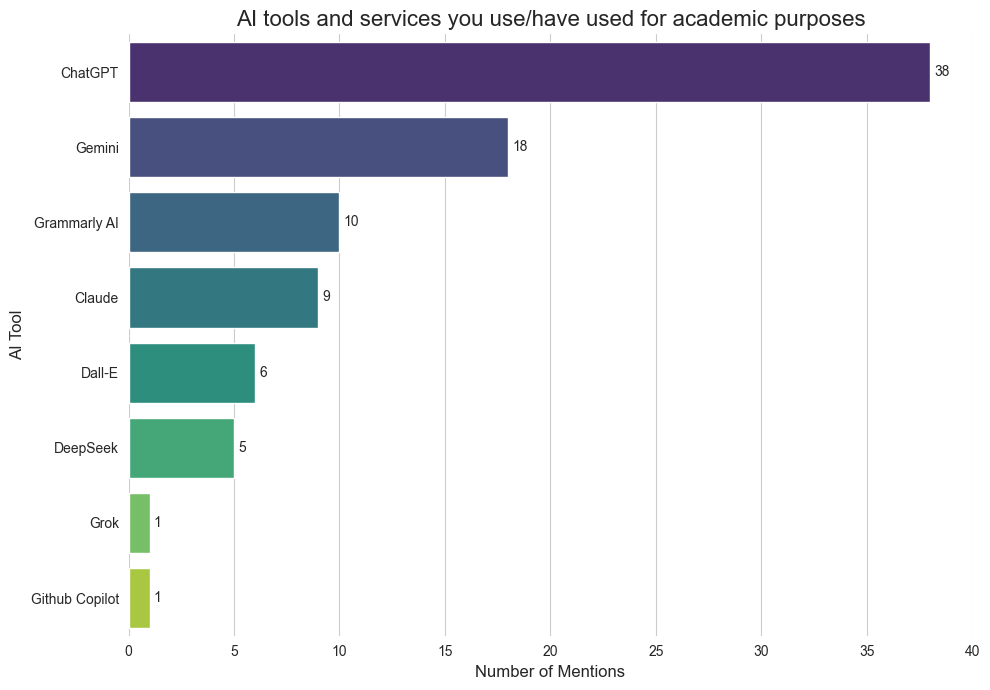
\includegraphics[width=0.7\textwidth]{fig3.png} % Replace with your figure file name
  \caption{A brief description of the figure.}
  \label{fig:example1}
\end{figure}

Breakdowns by academic major are presented in Figure 4. Among Engineering majors, 94.4\% (17 of 18) reported using ChatGPT, 38.9\% (7) used Gemini, and 27.8\% (5) used Claude. Among Liberal Arts and Sciences majors, all 11 respondents (100\%) reported using ChatGPT, while 45.5\% (5) used Gemini and 27.3\% (3) used Grammarly AI. Results for Business and Health Professions majors are also included but should be considered in light of the smaller sample sizes (n = 5 each). 

% Example of two subfigures side-by-side
\begin{figure}[htbp]
  \centering
  \begin{subfigure}[b]{0.45\textwidth}
    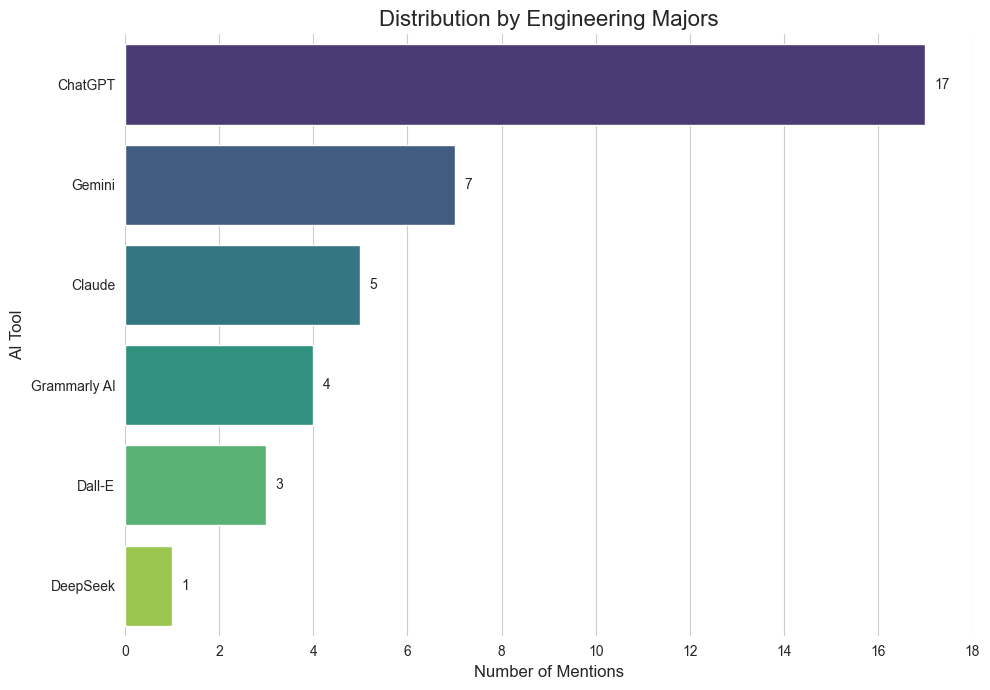
\includegraphics[width=\textwidth]{fig4-1.png} % Replace with your first subfigure file name
    %\caption{Description of subfigure (a)}
    \label{fig:subfig1a}
  \end{subfigure}
  \hfill % Add some horizontal space between the subfigures
  \begin{subfigure}[b]{0.45\textwidth}
    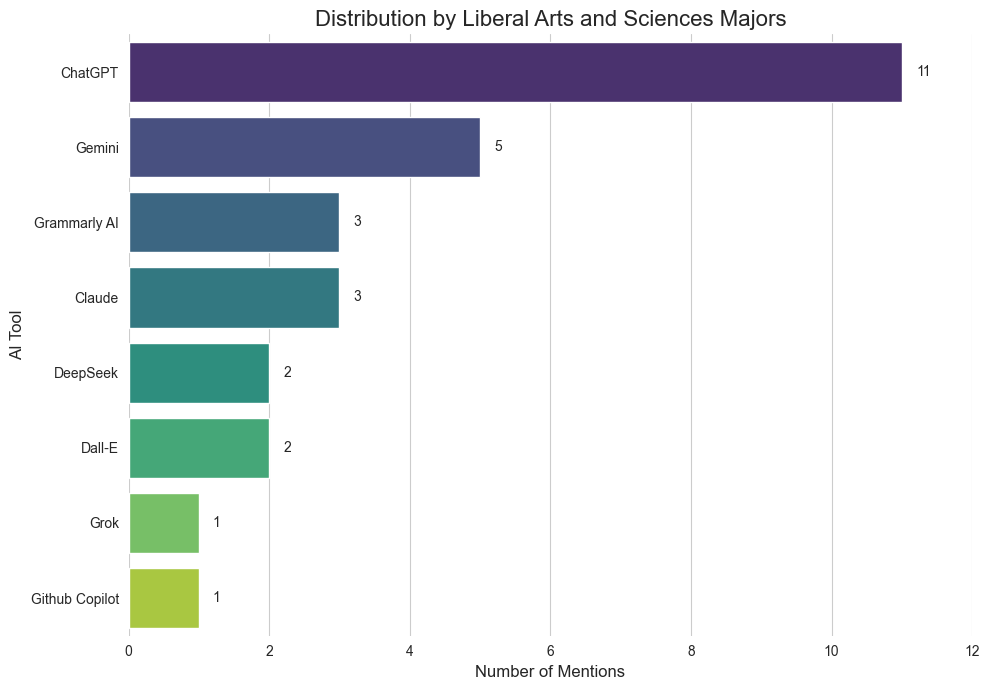
\includegraphics[width=\textwidth]{fig4-2.png} % Replace with your second subfigure file name
    %\caption{Description of subfigure (b)}
    \label{fig:subfig1b}
  \end{subfigure}
  \hfill % Add some horizontal space between the subfigures
  \begin{subfigure}[b]{0.45\textwidth}
    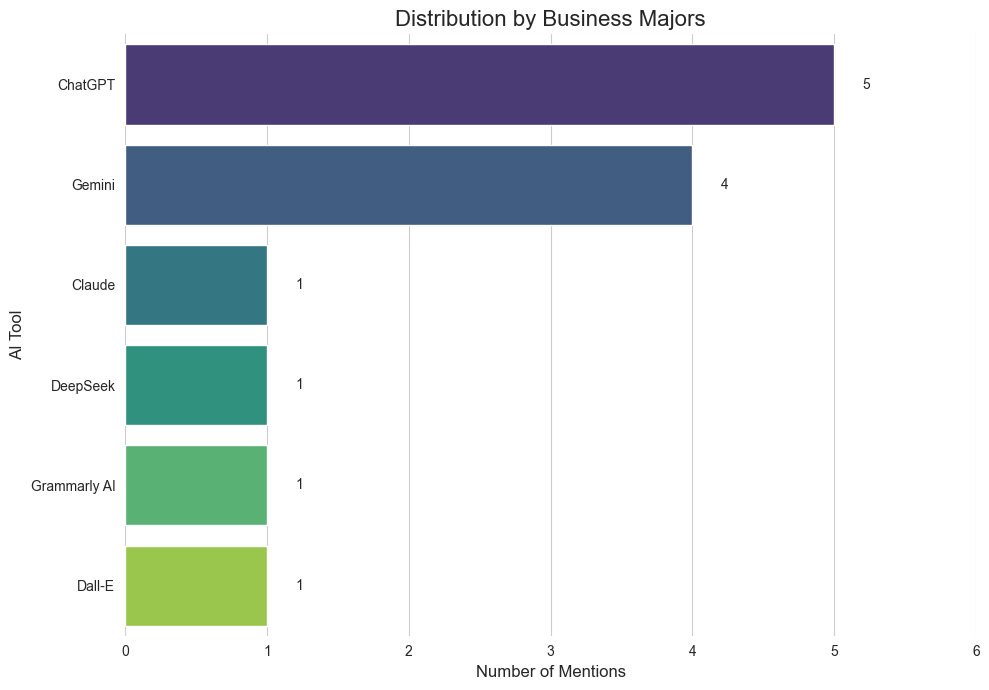
\includegraphics[width=\textwidth]{fig4-3.png} % Replace with your second subfigure file name
    %\caption{Description of subfigure (b)}
    \label{fig:subfig1b}
  \end{subfigure}
  \hfill % Add some horizontal space between the subfigures
  \begin{subfigure}[b]{0.45\textwidth}
    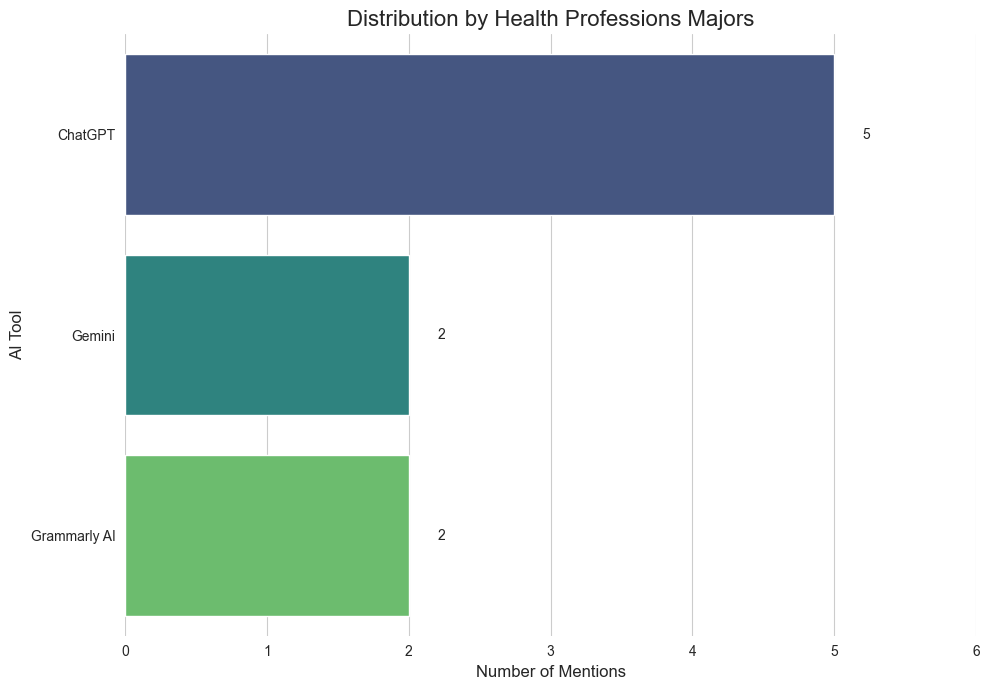
\includegraphics[width=\textwidth]{fig4-4.png} % Replace with your second subfigure file name
    %\caption{Description of subfigure (b)}
    \label{fig:subfig1b}
  \end{subfigure}
  \caption{Overall caption for the two subfigures.}
  \label{fig:subfigures1}
\end{figure}

Participants were also asked to select academic tasks for which they use AI tools. The most commonly selected task was writing and editing, chosen by 87\% (34 respondents). Other frequently selected tasks included research and information gathering (74\%), studying and note-taking (62\%, 24 respondents), math and problem solving (59\%, 23 respondents), and career and professional development (46\%, 18 respondents). Coding was selected by 41\% (16 respondents), productivity and organization by 26\% (10 respondents), data analysis and visualization by 21\% (8 respondents), and presentation and content creation by 18\% (7 respondents). These task-based results are broken down by major in Figure 6. 

\begin{figure}[htbp]
  \centering
  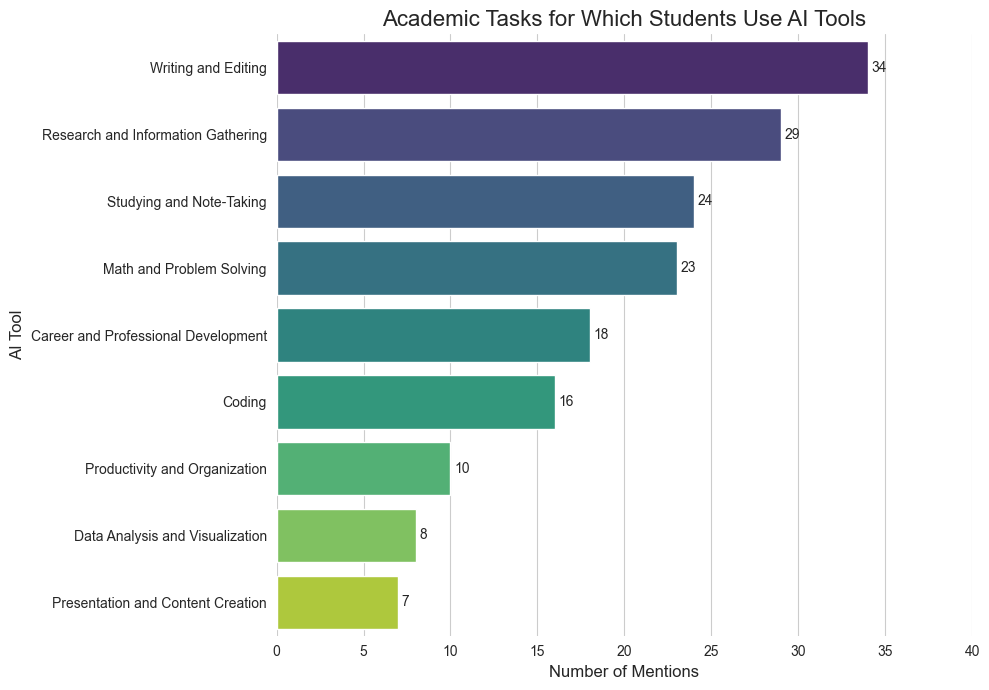
\includegraphics[width=0.5\textwidth]{fig5.png} % Replace with your figure file name
  \caption{A brief description of the figure.}
  \label{fig:example1}
\end{figure}


% Example of two subfigures side-by-side
\begin{figure}[htbp]
  \centering
  \begin{subfigure}[b]{0.45\textwidth}
    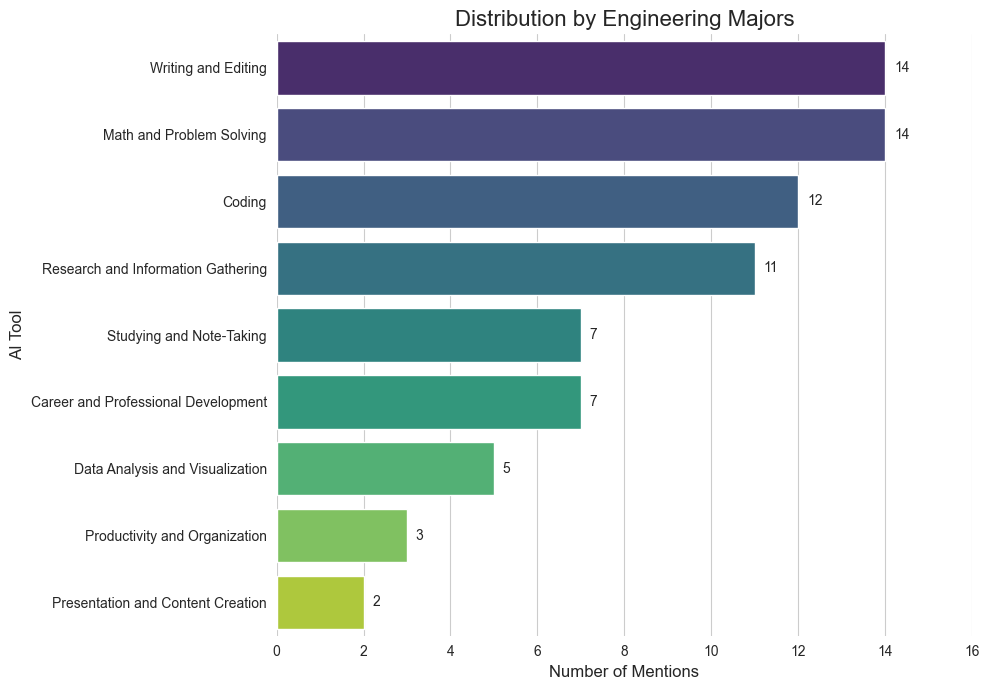
\includegraphics[width=\textwidth]{fig6-1.png} % Replace with your first subfigure file name
    %\caption{Description of subfigure (a)}
    \label{fig:subfig1a}
  \end{subfigure}
  \hfill % Add some horizontal space between the subfigures
  \begin{subfigure}[b]{0.45\textwidth}
    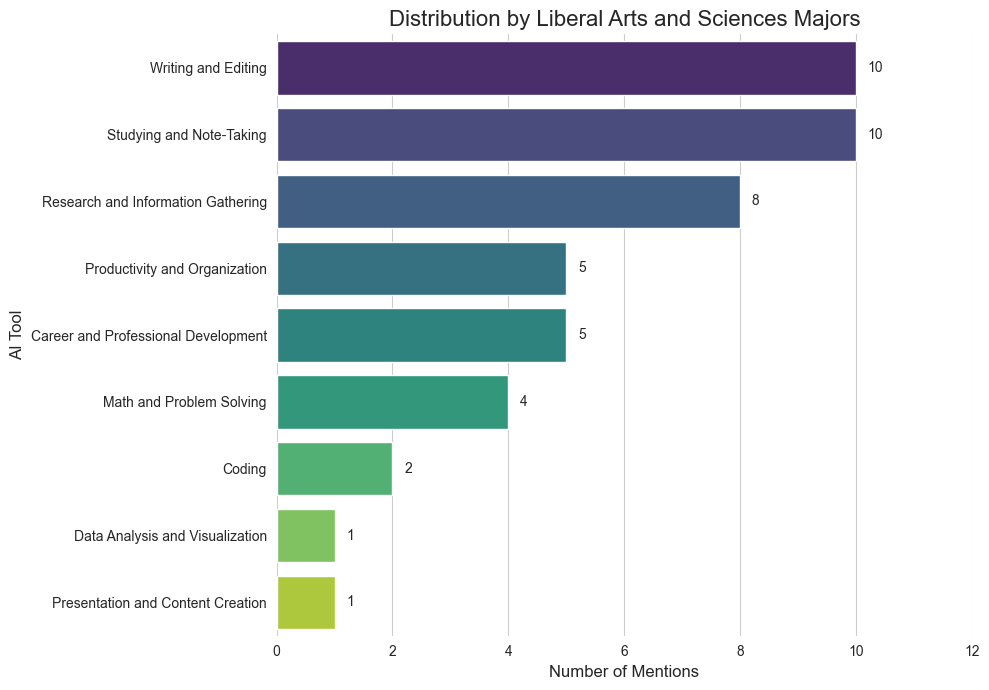
\includegraphics[width=\textwidth]{fig6-2.png} % Replace with your second subfigure file name
    %\caption{Description of subfigure (b)}
    \label{fig:subfig1b}
  \end{subfigure}
  \hfill % Add some horizontal space between the subfigures
  \begin{subfigure}[b]{0.45\textwidth}
    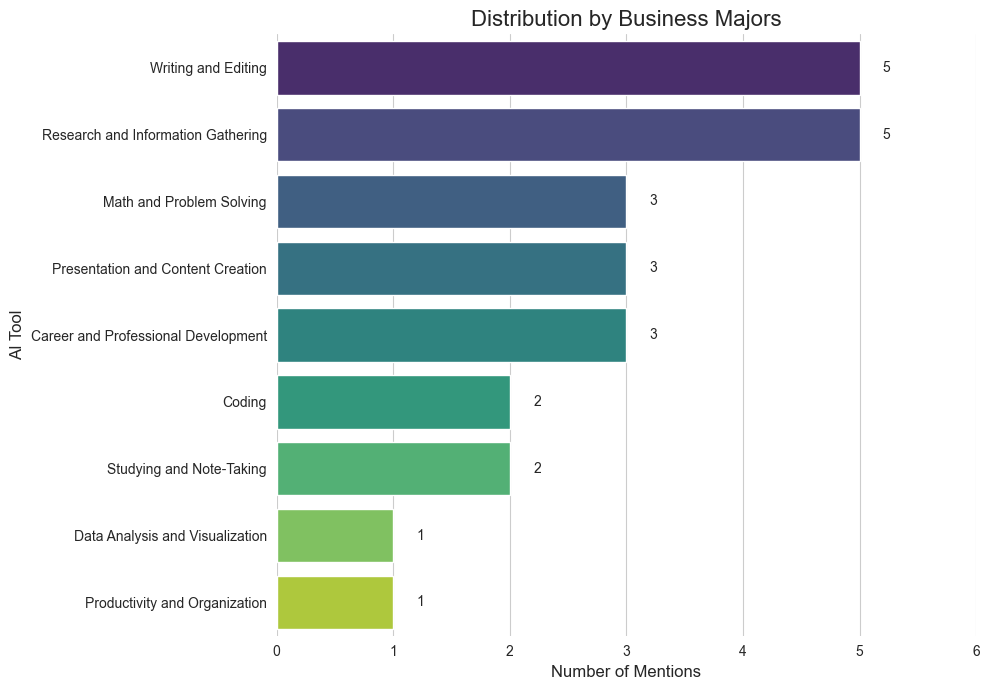
\includegraphics[width=\textwidth]{fig6-3.png} % Replace with your second subfigure file name
    %\caption{Description of subfigure (b)}
    \label{fig:subfig1b}
  \end{subfigure}
  \hfill % Add some horizontal space between the subfigures
  \begin{subfigure}[b]{0.45\textwidth}
    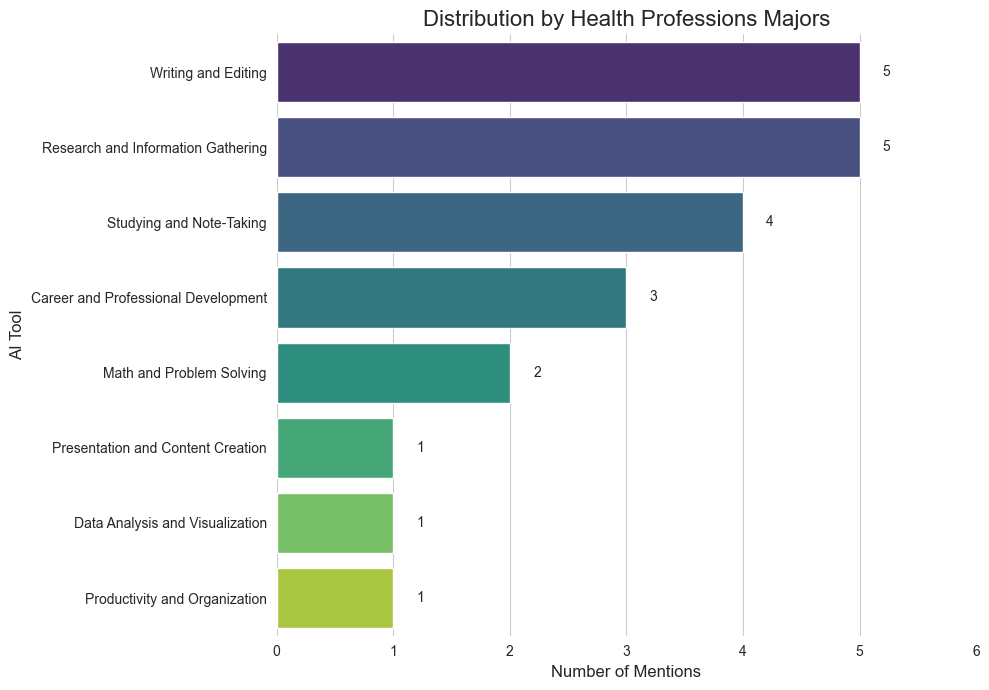
\includegraphics[width=\textwidth]{fig6-4.png} % Replace with your second subfigure file name
    %\caption{Description of subfigure (b)}
    \label{fig:subfig1b}
  \end{subfigure}
  \caption{Overall caption for the two subfigures.}
  \label{fig:subfigures1}
\end{figure}


The survey also included three attitudinal statements, each rated on a Likert scale from “strongly disagree” to “strongly agree.” In response to the statement “AI improves my learning experience as a student,” 19 participants strongly agreed, 13 somewhat agreed, 4 neither agreed nor disagreed, 2 somewhat disagreed, and 1 strongly disagreed (Figure 7). For the statement “AI tools are accessible to me,” 23 participants strongly agreed, 15 somewhat agreed, and 2 neither agreed nor disagreed (Figure 8). Responses to the statement “AI tools are more beneficial in my field of study compared to others” were more mixed: 17 selected “neither agree nor disagree,” 10 somewhat agreed, 9 strongly agreed, and 4 somewhat disagreed (Figure 9). A breakdown of responses by academic discipline is presented in the Discussion and Conclusion section.


\subsection{Textual Description of Results}
Describe the main findings in words.

\subsection{Figures}
\label{subsec:figures}
You can include figures in this subsection or create separate subsections for different sets of figures.

% Example of a single figure
\begin{figure}[htbp]
  \centering
  \includegraphics[width=0.7\textwidth]{example-image-a} % Replace with your figure file name
  \caption{A brief description of the figure.}
  \label{fig:example1}
\end{figure}

% Example of two subfigures side-by-side
\begin{figure}[htbp]
  \centering
  \begin{subfigure}[b]{0.45\textwidth}
    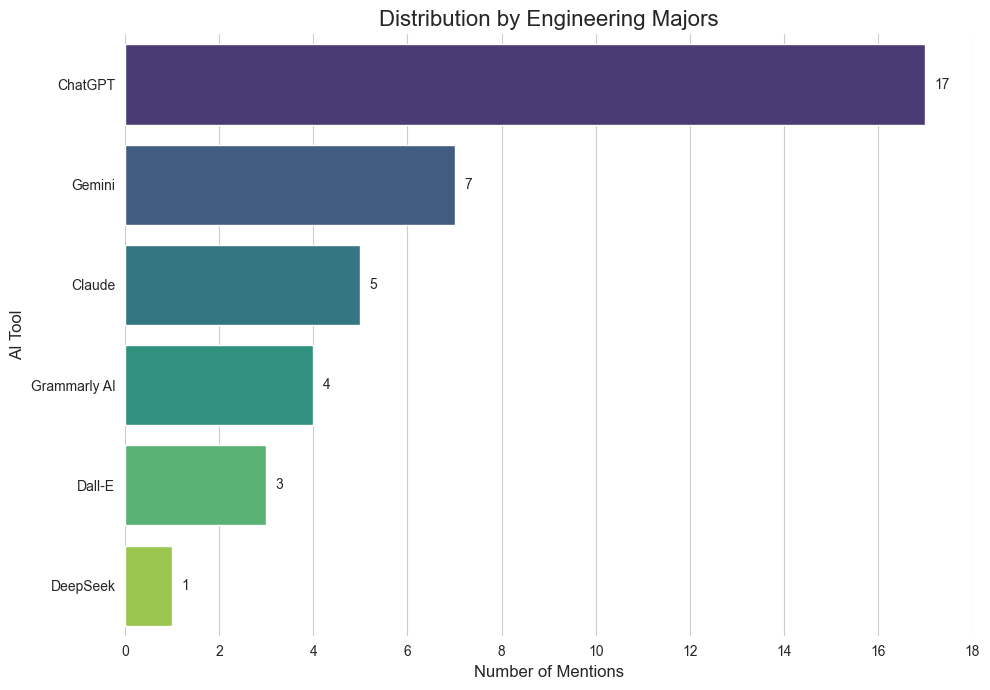
\includegraphics[width=\textwidth]{fig4-1.png} % Replace with your first subfigure file name
    \caption{Description of subfigure (a)}
    \label{fig:subfig1a}
  \end{subfigure}
  \hfill % Add some horizontal space between the subfigures
  \begin{subfigure}[b]{0.45\textwidth}
    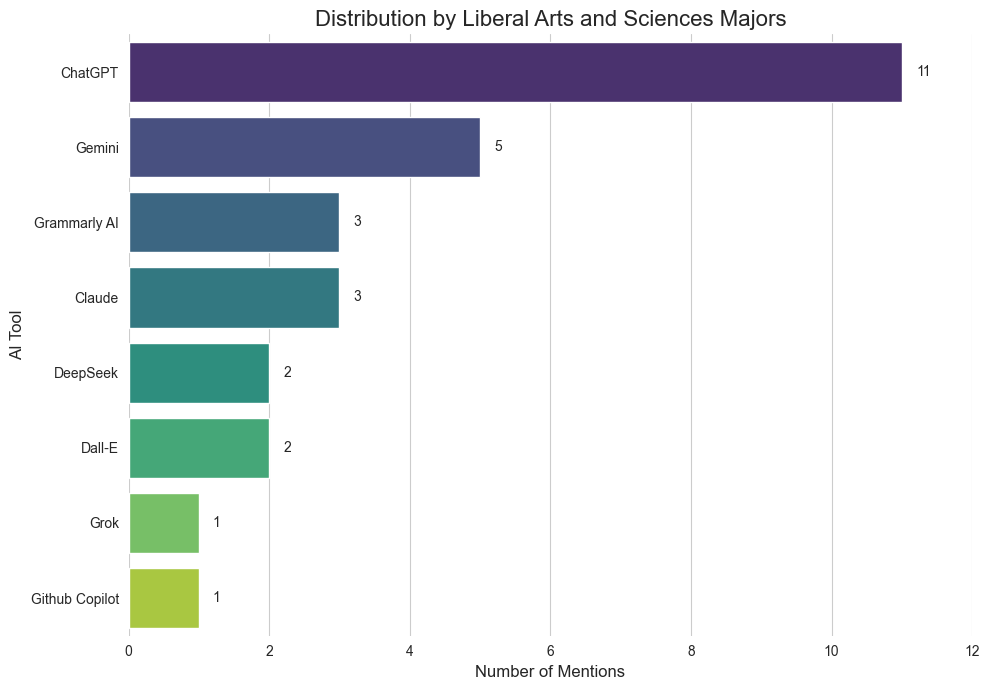
\includegraphics[width=\textwidth]{fig4-2.png} % Replace with your second subfigure file name
    \caption{Description of subfigure (b)}
    \label{fig:subfig1b}
  \end{subfigure}
  \hfill % Add some horizontal space between the subfigures
  \begin{subfigure}[b]{0.45\textwidth}
    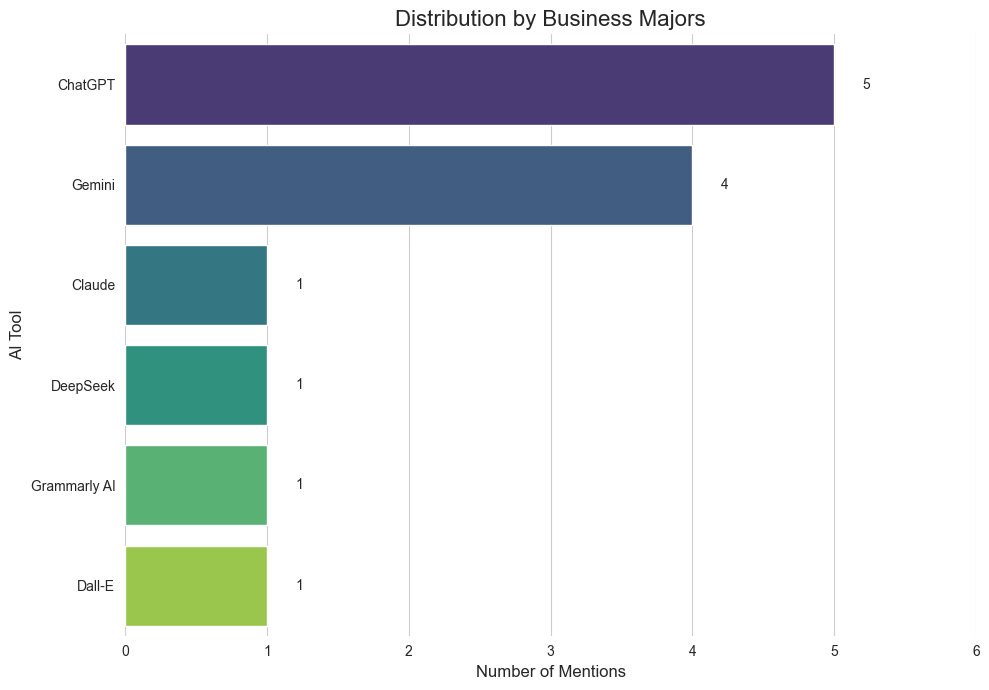
\includegraphics[width=\textwidth]{fig4-3.png} % Replace with your second subfigure file name
    \caption{Description of subfigure (b)}
    \label{fig:subfig1b}
  \end{subfigure}
  \hfill % Add some horizontal space between the subfigures
  \begin{subfigure}[b]{0.45\textwidth}
    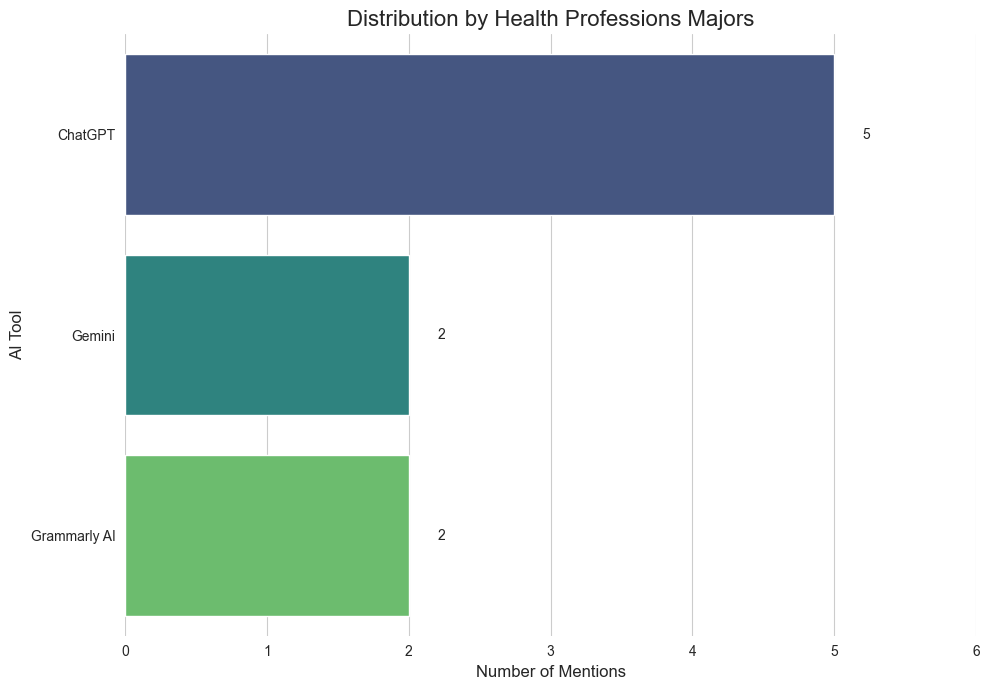
\includegraphics[width=\textwidth]{fig4-4.png} % Replace with your second subfigure file name
    \caption{Description of subfigure (b)}
    \label{fig:subfig1b}
  \end{subfigure}
  \caption{Overall caption for the two subfigures.}
  \label{fig:subfigures1}
\end{figure}

% --- Discussion ---
\section{Discussion}
\label{sec:discussion}
In this section, you interpret and discuss the results presented in the previous section. Relate your findings back to the research question and the existing literature. Discuss the implications of your findings, any limitations of your study, and potential avenues for future research.

% --- Conclusion ---
\section{Conclusion}
\label{sec:conclusion}
Summarize the main findings and conclusions of your research. Briefly reiterate the significance of your work.

% --- Acknowledgements (Optional) ---
\section*{Acknowledgements}
You can acknowledge individuals or organizations that provided support for your research.

% --- References ---
\section*{References}
\label{sec:references}
List all the sources you cited in your report using a consistent citation style.

% Example using a simple \thebibliography environment:
\begin{thebibliography}{99}
  \bibitem{AuthorYear} Author, A. (Year). \textit{Title of the book or article}. Publisher or Journal Name, Volume(Issue), pages.
  % Add more references here
\end{thebibliography}

% --- Appendices (Optional) ---
\appendix
\section{Appendix A: Supplementary Material}
Include any supplementary materials here.

% --- End Document ---
\end{document}